\title{Istanbul Technical University}
\author{
	BLG527E Machine Learning(HW4)\\
	Aydin Ayanzadeh \\
	Department of Computer Engineering\\
	Email:ayanzadeh17@itu.edu.tr\\
	student ID: 504161503 }
	
\date{\today}

\documentclass[12pt]{article}
\usepackage{graphicx}
\usepackage{mathtools}
\usepackage{hyperref}
\usepackage[margin=1in, paperwidth=8.5in, paperheight=11in]{geometry}

\begin{document}
	\maketitle
	
	\paragraph{Q1a,b} In figure1, histogram of means for 10 and 100 samples has plotted,(left plot(blue plot) is the histogram of means for 100 samples; right plot(pink plot) is the histogram of means for 10 samples) 
	
	\begin{figure}[h]
		
		\centerline{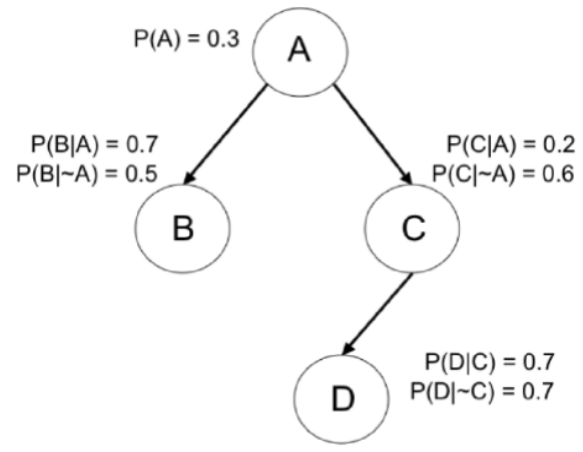
\includegraphics[width=3.5in]{22.png}}
		\caption{ Bayesian network(Graphical Model) }
		\label{fig1:Histograms pw1=pw2}
		
	\end{figure}
	
	$a) p(A,B,C,D)=P(D|c)P(C|A)P(B|A)P(A) $ $=0.7*0.2*0.7*0.3=0.0294$\\
	
	$b) p(A|B)=\dfrac{P(B,A)}{P(B)}=\frac{P(B|A)P(A)}{P(B|A)P(A)+P(B|~A)P(~A)}$\\\\
	
	 $=\frac{0.7*0.3}{0.7*0.3+0.5*0.7}=0.375$\\
	 
	 
	 $c) P(C|B)=\dfrac{P(C,B)}{P(B)}=\frac{P(B)P(C)}{P(B)}=P(C)$\\
	\paragraph{Q1C}
	 The \textit{central limit theorem} states that if we have  large random samples from the population(from any distribution
	 with means of $\mu$ and variance of $\sigma^{2}$ ), then the distribution of these sample means will be approximately normally distributed. In central limit theorem if we have N samples from a  distribution with variance and mean of $\sigma^2$ and $\mu$(N=10,N=100) ; we compute the mean of samples(mi = mean(Xi)) and repeat this for the determined time(number of repetition is determined 500).According to the results, we can reaching an agreement that by increasing the number of N the distribution get more closer the normal distribution with means of $\mu$ and $\sigma$. \\ In the following, i want to explain the difference and similarities of two plots.\\\\
	
	\textit{\textbf{Differences}}
\begin{itemize}
	\item the histogram that have N=100 sample is more similar to Normal distribution than the samples with N=10.
	\item  variances is the second difference of plots. when N increases the differences will be less meaningful.Therefore, the variance of histograms for N = 100 are closer to each other than histograms for N = 10.
\\

	
\end{itemize}
	
		\textit{\textbf{Similarities}}
		\begin{itemize}
			\item Both of plots looks like normal distribution.
			\item The mean of all histograms are μ = 0 because the mean of distributions which we
			draw random samples from equal 0.
		
		\end{itemize}
		\paragraph{Q2a}	The information that has given in the problem and discriminant functions is listed below:	
				
	$$	p(x|C1) = N(0,1)$$ $$p(x|C2) = N(1,2)$$
	$$c1:x^{i}\sim N(\mu_{1},\sigma_{1})$$ 
		$$c2:x^{i}\sim N(\mu_{2},\sigma_{2})$$	
		$$g_{1}(x)=ln(p(x|c{i}))+p(c_{i})$$
		$P(c1)=p(c2)=0.5$

			we derive the equation for class1 and class 2 according the above information.
			$$p(x|c{i})=\frac{1}{\sqrt{2\pi\sigma}}exp(-\frac{(x-{\mu_{i}})^{2}}{2\sigma_{i}^{2}})$$
			after plugging the likelihoods in discriminant function , we will have discriminant function for g1:

		$$g_{1}(x)=ln(\frac{1}{\sqrt{2\pi\sigma_{1}}})exp[\frac{-(x-\mu_{1})^{2}}{2\sigma_{1}^{2}}]+ln(p(w_{1}))$$
		
		after extending and simplifying the equation we will have discriminant functions for class1 and class2:


		
		$$g_{1}(x)=-\frac{1}{2}ln(2\pi)-ln(\sigma_{1})-(\frac{(x-\mu_{1})^{2}}{2\sigma_{1}^{2}})+ln(p(c_{1}))$$
		
		$$g_{2}(x)=-\frac{1}{2}ln(2\pi)-ln(\sigma_{2})-(\frac{(x-\mu_{2})^{2}}{2\sigma_{2}^{2}})+ln(p(c_{2}))$$
	
		
		
		
		\newpage		
		$$\sigma=\sqrt[3]{\dfrac{1}{N} \sum_{n=1}^{N} (P_{K}-E)^3 }$$
				
	\paragraph{Q2b} In this question we generate random datasets for likelihoods(i create two  random dataset with 300000 variables that has distributed based on the Gaussian function.) that has distributed according to the Gaussian. In Figure2, we plot the $P(C_{1}|x) and P(C_{2}|x)$ and density histogram of likelihood functions. Blue line is the likelihood of class1 and red line in the plot is the likelihood of class2. Moreover, in Figure3, we plots the posteriors of class with equal priors ( $P(c_{1})=p(c_{2})=0.5$) when we have one-dimensional inputs.
	

	\paragraph{Q2c} we can see the discriminant functions of class 1 and class2 in Figure4. for identifying the decision regions for two classes, we should find the separation surface of two classes. by putting the equivalent of two discriminant function, we can find the separation surface for them.
			$$g_{1}(x)=g_{2}(x)$$
			
			$$-\frac{1}{2}ln(2\pi)-ln(\sigma_{1})-(\frac{(x-\mu_{1}^{2})}{2\sigma_{1}^{2}})+ln(p(c_{1}))=-\frac{1}{2}ln(2\pi)-ln(\sigma_{2})-(\frac{(x-\mu_{2}^{2})}{2\sigma_{2}^{2}})+ln(p(c_{2}))$$ 
			
after extending and simplifying the equation, we will reach the second-degree polynomial function:		
		  $$(\frac{1}{2\sigma^{2}_{2}}-\frac{1}{2\sigma^{2}_{1}})x^{2}+(\frac{\mu_{1}}{2\sigma^{2}}_{1}-\frac{\mu_{2}}{\sigma^{2}}_{2})x+\frac{\mu^{2}_{2}}{2\sigma^{2}_{2}}-\frac{\mu^{2}_{1}}{2\sigma^{2}_{1}}+ln\frac{\sigma_{2}}{\sigma_{1}}+\frac{p(c_{1})}{p(c_{2})}=0$$
		  
		  
by plugging the number of $\sigma_{1},\sigma_{2},\mu_{1}, \mu_{1},\mu_{2},c_{1} and  c_{2}$ in the function, we will see that $\Delta\geq0$ so we have 2 discriminator for our discriminant function, after finding the roots of equation, we have x1=-1.84754498496518 and x2=1.18087831829851 is our point of discriminant. you can see the regions of classes in Figure4.we can also see the regions of classes by likelihoods of class more efficiently in Figure5.	
			
	
								
								\paragraph{Q2d}	when $p(c_{2})=0.8$ and $p(c_{1})=0.2 $,   $\dfrac{p(c_{1})}{p(c_{2})}$ will be less than zero, in this condition, delta of equation of intersection of g1 and g2 will be less than zero	($\Delta=b^{2}-4ac<0$) therefore,we do not have any intersection region and x to discriminate our classes.In this case we just have one region to our classes, the reason that we choose just one region to our spaces is that when $ p(c_{2}) $ increases to 0.8, g2 will cover g1 function in all regions. Hence, this model will recognize the each input to R2. In figure6 you see the discriminant functions of g1 and g2 and regions of classes.
								
						



$$\varDelta\eta$$

	\newpage
		

\end{document}

